\chapter{Theoretische Vorbemerkung}

Im ersten Teil dieses Kapitels werden zunächst einmal die Grundlagen zu Augmented Reality beschrieben, wie diese Technologie einzuordnen ist, welche technischen Anforderungen ein Augmented Reality System hat und wo typische Einsatzszenarien liegen.

\section{Augmented Reality}

Augmented Reality (AR) ist eine Klasse aus dem Realitäts-Virtualitäts-Kontinuum von \cite{milgram1995augmented}, zu finden in Abbildung \ref{fig:virtual-continuum}, welche reale und virtuelle Objekte in einer realen Umgebung kombiniert. Diese virtuellen Objekte sind in der realen Umgebung idealerweise fest lokalisiert und fügen sich somit in das reale Erscheinungsbild ein. Typischerweise sind AR Anwendungen interaktiv, und stellen die virtuellen Objekte in Echtzeit und dreidimensional in der realen Welt dar. Für die Definition von AR Anwendungen gibt es zudem keine Limitierung für die Darstellungstechnologie, wie zum Beispiel das Projekt Tango Tablett oder einem Head-Mounted Display. AR beschränkt sich zudem nicht auf den angesprochenen Sinn - so sind zum Beispiel AR Anwendungen mit visueller, olfaktorischer oder taktiler Umsetzung möglich. 

Virtuel Reality (VR) oder auch Virtual Environment hingegen kapselt sich von der realen Umgebung ab und bietet Interaktionen in reinen virtuellen Umgebungen. VR konnte sich im Gegensatz zu AR deutlich schneller Entwickeln, da die technologischen Anforderungen an AR deutlich höher sind. \citep{van2010survey}


\begin{figure}
  \centering
	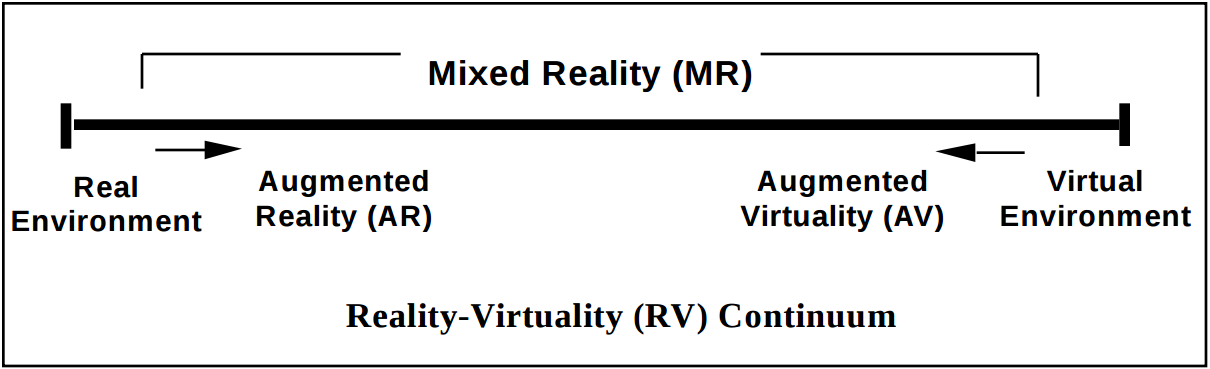
\includegraphics[width=0.85\textwidth]{content/images/virtual-continuum.png} 
  \caption{Vereinfachte Darstellung des Realitäts-Virtualitäts-Kontinuum von \citet*{milgram1995augmented}}
  \label{fig:virtual-continuum}
\end{figure}

\subsection{Technische Anforderungen}

Dieser Abschnitt widmet sich den technischen Anforderungen an Augmented Reality, indem die potentiellen Display Technologien beschrieben werden, mögliche Trackingverfahren erläutern werden und zuletzt die Systeme bestimmt werden, mit denen ein Nutzer mit dem AR System interagieren kann.

\subsubsection{Display Technologie}

Der erste wichtige Teil der technologischen Anforderungen an AR sind visuelle Anzeigen (visual displays), welche sich nach \citet{van2010survey}
in diesem Anwendungsfall zunächst in drei Arten der Darstellung unterteilen und zudem unterschiedlich positioniert werden können. Die einfachste und günstigste Art der visuellen Darstellung in AR ist \enquote{video see-through}, wodurch die reale Umgebung durch eine Video Aufnahme ersetzt wird und die virtuellen Objekte digital in die Video Aufnahme gerendert werden. Das bietet außerdem die Möglichkeit Objekte aus der realen Umgebung zu entfernen oder zu ändern oder anhand der Luminanz Information vom Video das Rendering der virtuellen Objekte entsprechend an die Realität anzupassen.

Die nächste Möglichkeit zur Darstellung ist \enquote{optical see-through}, wodurch die virtuellen Objekte durch transparente Spiegel in das Sichtfeld des Betrachters gebracht werden. Anders als bei \enquote{video see-throught} bleibt die reale Auflösung für die visuelle Aufnahme des Betrachtes gleich und es können zudem keine Latenzprobleme beim Ändern des Betrachtungswinkels auftreten (parallax-effect).

Die dritte Möglichkeit ist die projizierte Darstellung, in der die Augmented Reality Überlagerung auf die realen Objekte projiziert werden. Diese Darstellung ermöglicht die Abdeckung vom gesamten Sichtfeld, benötigt aber eine entsprechende Kalibrierung bei Umgebungsänderungen.

Neben der Art der Darstellung können die Display Technologien laut \citet{azuma2001recent} anhand Ihrer Positionierung klassifiziert werden. Man unterscheidet zwischen am Kopf befestigten Displays (head-mounted), tragbare Displays  (hand-held) und räumlich positionierten Displays. Zu jeder dieser Displayarten gibt es wiederum unterschiedliche technische Umsetzungen mit ihren spezifischen Vor- und Nachteilen bezüglich ihrer Anwendungsszenarien.

\subsubsection{Tracking Technologien}

Um eine virtuelle Projektion im realen Raum zu realisieren muss zunächst die Position und gegebenenfalls relative Positionsänderung des Displays bestimmt werden, auch \enquote{augmented reality registration} genannt. Man spricht dabei üblichweise von den \enquote{six degrees of freedom (6DOF)}, der Position im Raum (x, y, z) und der Orientierung (yaw, pitch, roll). 



Frühe Techniken für die Registrierung benötigten eine speziell vorbereitete Räumlichkeit, denn sie basierten auf mechanischen, magnetischen oder Ultraschall Sensoren um die Position zu bestimmen. Diese Sensoren sind zwar immer noch im Einsatz und bilden auch den Grundstein für AR und VR Forschung, sind aber praktisch gesehen zu komplex und aufwändig für die meisten Anwendungsfälle. \citep{van2010survey} 

Für ein grobes Positions-Tracking, vor allem auch außerhalb von Gebäuden wird GPS genutzt. Für großräumliche Anwendung ist GPS mit einer Varianz von 10-15 Metern durchaus praktikabel. Zum Beispiel um sichtbare Flugzeuge oder Sterne zu identifizieren. Innerhalb von Gebäuden basiert die grobe Positionierung laut \citet{van2010survey} oft auf verfügbaren Wifi Access Points oder RFID Markern. \citet{lamarca2005place} demonstrieren hierzu auch die Möglichkeit diese Technologie für grobe Lokalisation außerhalb von Gebäuden einzusetzen.

Optische Tracking Verfahren basierend auf Bildverarbeitung bieten  (Seite 7)
Optische Sensoren
Hybride mit Trägheits Snesoren!


